\documentclass[12pt,a4paper]{article}
\usepackage{amsmath, amssymb, geometry, booktabs, xcolor, hyperref,
            listings, pgfplots, tcolorbox, enumitem, fancyhdr, tikz, array}
\geometry{margin=2.5cm}
\pgfplotsset{compat=1.18}
\tcbuselibrary{skins, breakable}

\newtcolorbox{curiositybox}[1]{colback=yellow!10, colframe=orange!80!black, fonttitle=\bfseries, title=#1, breakable}
\newtcolorbox{infobox}[1]{colback=blue!5, colframe=blue!60!black, fonttitle=\bfseries, title=#1, breakable}
\newtcolorbox{mistakebox}[1]{colback=red!5, colframe=red!60!black, fonttitle=\bfseries, title=#1, breakable}
\newtcolorbox{learnbox}[1]{colback=green!5, colframe=green!60!black, fonttitle=\bfseries, title=#1, breakable}

\lstset{language=Python, basicstyle=\ttfamily\small, keywordstyle=\color{blue},
        commentstyle=\color{gray}, stringstyle=\color{orange},
        showstringspaces=false, numbers=left, numberstyle=\tiny,
        breaklines=true, frame=single}

\pagestyle{fancy}
\fancyhf{}
\lhead{Topic 09: Laplace Transform of Integrals}
\rhead{Unit IV --- Laplace Transforms}
\cfoot{\thepage}

\title{Topic 09: Laplace Transform of Integrals \\
       \large Unit IV --- Laplace Transforms}
\author{23A54201 --- Mathematics IV (Transform Techniques) \\
        JNTUA College of Engineering (Autonomous)}
\date{}

\begin{document}
\maketitle
\tableofcontents
\newpage

%% -------------------------------------------------------
\section{Opening Hook}
%% -------------------------------------------------------

\begin{curiositybox}{Hook}
Topic 08 showed you something remarkable: differentiation in the $t$-domain becomes
multiplication by $s$ in the $s$-domain. Now here is the perfect companion result:
integration in the $t$-domain becomes division by $s$. So the entire calculus ---
differentiation and integration --- maps to simple arithmetic in the $s$-domain.
Multiply for derivatives, divide for integrals. This topic proves the division result and
shows you how to use it to handle integral equations and accumulation problems.
\end{curiositybox}

%% -------------------------------------------------------
\section{Why This Topic Exists}
%% -------------------------------------------------------

Before we begin, here is the honest answer to why you are reading this\ldots{}
Integral equations appear in every branch of engineering. In electrical engineering the
charge accumulated on a capacitor is $q(t) = \int_0^t i(\tau)\,d\tau$, where $i(\tau)$
is the current. In mechanics the displacement of a particle is the time integral of its
velocity. In control systems the integral of an error signal drives an integral
controller. Without the Laplace transform of an integral you cannot solve any of these
problems algebraically.

\begin{center}
\begin{tabular}{>{\bfseries}p{6.5cm} p{7.5cm}}
\toprule
Mistake & Consequence \\
\midrule
Not knowing the integral transform formula &
  Unable to solve integral equations using Laplace methods \\
\addlinespace
Forgetting to divide by $s$ (only multiplying) &
  Getting the derivative formula instead of the integral formula \\
\addlinespace
Confusing $\mathcal{L}\!\left\{\int_0^t f\right\}$ with $\mathcal{L}\{f\}/s$ as a
  general rule &
  Only correct if lower limit is $0$ --- wrong otherwise \\
\bottomrule
\end{tabular}
\end{center}

\begin{learnbox}{Key Takeaway}
Integrals in the $t$-domain become division by $s$ in the $s$-domain, provided the
lower limit of integration is $0$.
\end{learnbox}

%% -------------------------------------------------------
\section{You Already Know This (Intuition First)}
%% -------------------------------------------------------

Think about the relationship between multiplication and division in ordinary arithmetic.
When you know that differentiation corresponds to multiplication by $s$, it is completely
natural to expect that integration --- the inverse operation --- corresponds to division
by $s$. Just as the exponential and the logarithm are inverses (one ``goes up'' a level,
the other ``comes down''), differentiation and integration in the $t$-domain are inverses
of each other, and they correspond to multiplication and division by $s$ respectively.

Here is another way to feel this. Integration is an \emph{accumulation} operation: the
integral $\int_0^t f(\tau)\,d\tau$ is the running total of $f$ up to time $t$. In the
$s$-domain that accumulation over an extra variable corresponds to one more factor of
$1/s$ --- exactly the same way that $\int_0^\infty e^{-st}\,dt = 1/s$ introduces a factor
of $1/s$ for each integration over time. This is not a coincidence; it is the essence
of the transform.

%% -------------------------------------------------------
\section{The Main Theorem --- Transform of an Integral}
%% -------------------------------------------------------

\begin{infobox}{Theorem: Laplace Transform of an Integral}
\textbf{Theorem.} Let $f(t)$ be a piecewise continuous function of exponential order,
and let $\mathcal{L}\{f(t)\} = F(s)$. Then
\[
  \mathcal{L}\!\left\{\int_0^t f(\tau)\,d\tau\right\} = \frac{F(s)}{s}, \qquad s > 0.
\]

\bigskip
\noindent\textbf{Proof --- Method 1 (using the derivative formula from Topic 08).}

Define $g(t) = \int_0^t f(\tau)\,d\tau$. By the Fundamental Theorem of Calculus,
$g'(t) = f(t)$. Also note $g(0) = \int_0^0 f(\tau)\,d\tau = 0$.

By the Laplace derivative formula (Topic 08):
\[
  \mathcal{L}\{g'(t)\} = s\,G(s) - g(0) = s\,G(s) - 0 = s\,G(s).
\]
But $g'(t) = f(t)$, so $\mathcal{L}\{g'(t)\} = \mathcal{L}\{f(t)\} = F(s)$.

Therefore $F(s) = s\,G(s)$, which gives
\[
  G(s) = \frac{F(s)}{s}, \quad \text{i.e.,} \quad
  \mathcal{L}\!\left\{\int_0^t f(\tau)\,d\tau\right\} = \frac{F(s)}{s}. \qquad \square
\]

\bigskip
\noindent\textbf{Proof --- Method 2 (direct --- change of order of integration).}

Starting from the definition:
\[
  \mathcal{L}\!\left\{\int_0^t f(\tau)\,d\tau\right\}
  = \int_0^\infty e^{-st}\!\left[\int_0^t f(\tau)\,d\tau\right] dt.
\]
The region of integration in the $(\tau, t)$-plane is $\{0 \leq \tau \leq t < \infty\}$.
Reversing the order of integration (holding $\tau$ fixed and integrating $t$ from $\tau$
to $\infty$ first, then $\tau$ from $0$ to $\infty$):
\[
  = \int_0^\infty f(\tau)\!\left[\int_\tau^\infty e^{-st}\,dt\right] d\tau.
\]
Evaluate the inner integral:
\[
  \int_\tau^\infty e^{-st}\,dt = \left[\frac{e^{-st}}{-s}\right]_\tau^\infty
  = 0 - \frac{e^{-s\tau}}{-s} = \frac{e^{-s\tau}}{s}.
\]
Substituting back:
\[
  = \int_0^\infty f(\tau)\cdot\frac{e^{-s\tau}}{s}\,d\tau
  = \frac{1}{s}\int_0^\infty e^{-s\tau} f(\tau)\,d\tau = \frac{F(s)}{s}. \qquad \square
\]
\end{infobox}

\begin{learnbox}{What Did We Learn?}
Both proofs confirm $\mathcal{L}\!\left\{\int_0^t f(\tau)\,d\tau\right\} = F(s)/s$.
Method~1 is slick (one line using the derivative formula). Method~2 is foundational
(shows the geometry of interchanging integration order).
\end{learnbox}

%% -------------------------------------------------------
\section{Inverse Form}
%% -------------------------------------------------------

\begin{infobox}{Inverse Form of the Integral Theorem}
Taking the inverse Laplace transform of both sides of the main theorem:
\[
  \mathcal{L}^{-1}\!\left\{\frac{F(s)}{s}\right\} = \int_0^t f(\tau)\,d\tau,
\]
where $f(t) = \mathcal{L}^{-1}\{F(s)\}$.

\medskip
\noindent\textbf{Interpretation.} Whenever you see a transform of the form $F(s)/s$ (i.e.,
$F(s)$ multiplied by $1/s$), the inverse transform is the running integral of $f(t)$
from $0$ to $t$. The ``bonus $1/s$'' means: integrate once.

\medskip
\noindent\textbf{Worked Example.} Find $\mathcal{L}^{-1}\!\left\{\dfrac{1}{s^3}\right\}$.

Write $\dfrac{1}{s^3} = \dfrac{1/s^2}{s}$. We know $\mathcal{L}^{-1}\{1/s^2\} = t$.
By the inverse form, the extra $1/s$ means integrate:
\[
  \mathcal{L}^{-1}\!\left\{\frac{1}{s^3}\right\} = \int_0^t \tau\,d\tau
  = \left[\frac{\tau^2}{2}\right]_0^t = \frac{t^2}{2}.
\]
\textbf{Verification.} $\mathcal{L}\!\left\{\dfrac{t^2}{2}\right\}
= \dfrac{1}{2}\cdot\dfrac{2!}{s^3} = \dfrac{1}{s^3}$. $\checkmark$
\end{infobox}

\begin{learnbox}{What Did We Learn?}
A factor of $1/s$ in the $s$-domain corresponds to one integration in the $t$-domain.
Use this to invert transforms that have an ``extra'' $1/s$ factor.
\end{learnbox}

%% -------------------------------------------------------
\section{Repeated Integration}
%% -------------------------------------------------------

\begin{infobox}{Repeated Integration Formula}
\textbf{Theorem.} If $\mathcal{L}\{f(t)\} = F(s)$, then applying the integral theorem
$n$ times:
\[
  \mathcal{L}\!\left\{
    \underbrace{\int_0^t\!\int_0^{t_1}\!\cdots\!\int_0^{t_{n-1}}}_{n\text{ times}}
    f(t_n)\,dt_n\cdots\,dt_1
  \right\} = \frac{F(s)}{s^n}.
\]

\medskip
\noindent\textbf{Case $n = 2$ (explicit derivation).} Let
$g(t) = \int_0^t f(\tau)\,d\tau$. By the single-integral theorem:
\[
  \mathcal{L}\{g(t)\} = \frac{F(s)}{s}.
\]
Now define $h(t) = \int_0^t g(u)\,du$. Applying the theorem again with $g$ in place
of $f$ and $G(s) = F(s)/s$ in place of $F(s)$:
\[
  \mathcal{L}\{h(t)\} = \frac{G(s)}{s} = \frac{F(s)/s}{s} = \frac{F(s)}{s^2}.
\]
But $h(t) = \int_0^t\!\int_0^{t_1} f(\tau)\,d\tau\,dt_1$, so:
\[
  \mathcal{L}\!\left\{\int_0^t\!\int_0^{t_1} f(\tau)\,d\tau\,dt_1\right\}
  = \frac{F(s)}{s^2}.
\]
Each additional integration multiplies the denominator by one more factor of $s$.
\end{infobox}

\begin{learnbox}{What Did We Learn?}
$n$ nested integrations from $0$ to $t$ divide the transform by $s^n$.
Each ``layer'' of integration adds one factor of $1/s$ in the $s$-domain.
\end{learnbox}

%% -------------------------------------------------------
\section{Application --- Integral Equations}
%% -------------------------------------------------------

\begin{infobox}{Solving Integral Equations with Laplace Transforms}

\noindent\textbf{Background.} A Volterra integral equation involves an unknown function
$f(t)$ under an integral sign. The Laplace transform converts such equations to
algebraic equations in $F(s)$, which can be solved directly.

\medskip
\noindent\textbf{Volterra Equation of the First Kind.}
Given: $\displaystyle\int_0^t f(\tau)\,d\tau = g(t)$.

Take $\mathcal{L}$ of both sides:
\[
  \frac{F(s)}{s} = G(s) \implies F(s) = s\,G(s) \implies f(t) = g'(t).
\]
The integral equation is solved by differentiation --- an elegant result.

\medskip
\noindent\textbf{Volterra Equation of the Second Kind.}
Solve: $f(t) + \displaystyle\int_0^t f(\tau)\,d\tau = 1$.

\textbf{Step 1.} Take $\mathcal{L}$ of both sides:
\[
  F(s) + \frac{F(s)}{s} = \frac{1}{s}.
\]
\textbf{Step 2.} Factor out $F(s)$:
\[
  F(s)\!\left(1 + \frac{1}{s}\right) = \frac{1}{s}
  \implies F(s)\cdot\frac{s+1}{s} = \frac{1}{s}.
\]
\textbf{Step 3.} Solve for $F(s)$:
\[
  F(s) = \frac{1}{s}\cdot\frac{s}{s+1} = \frac{1}{s+1}.
\]
\textbf{Step 4.} Invert:
\[
  f(t) = \mathcal{L}^{-1}\!\left\{\frac{1}{s+1}\right\} = e^{-t}.
\]
\textbf{Verification.} $f(t) = e^{-t}$, so $\int_0^t e^{-\tau}\,d\tau = 1 - e^{-t}$.
Then $f(t) + \int_0^t f(\tau)\,d\tau = e^{-t} + (1 - e^{-t}) = 1$. $\checkmark$
\end{infobox}

\begin{learnbox}{What Did We Learn?}
The Laplace transform converts a Volterra integral equation into a simple algebraic
equation. For the first kind: $F(s) = s\,G(s)$, so $f = g'$. For the second kind:
factor out $F(s)$ and solve.
\end{learnbox}

\subsection*{Graphical Illustration}

Below is a plot of the solution $f(t) = e^{-t}$ and its running integral
$\int_0^t e^{-\tau}\,d\tau = 1 - e^{-t}$, which together sum to $1$, confirming the
integral equation.

\begin{center}
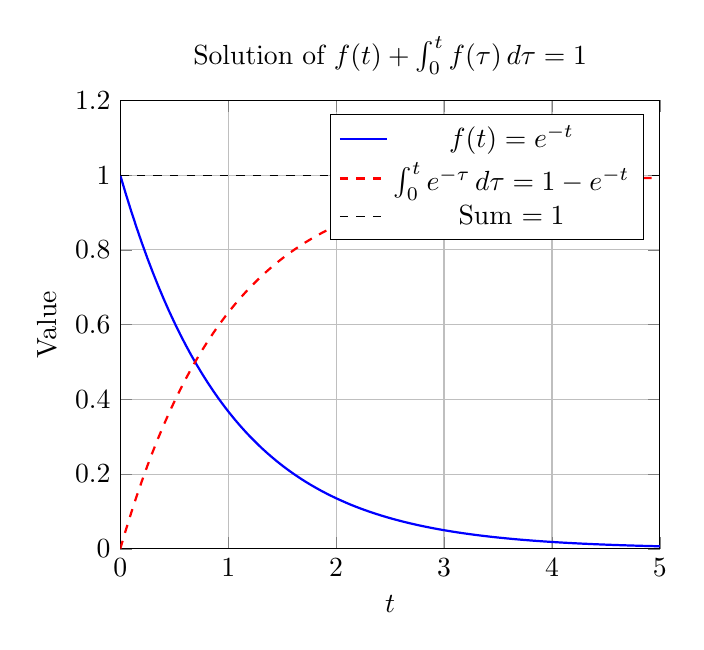
\begin{tikzpicture}
\begin{axis}[
  xlabel={$t$},
  ylabel={Value},
  xmin=0, xmax=5,
  ymin=0, ymax=1.2,
  grid=major,
  legend pos=north east,
  title={Solution of $f(t) + \int_0^t f(\tau)\,d\tau = 1$}
]
\addplot[blue, thick, domain=0:5, samples=100] {exp(-x)};
\addlegendentry{$f(t) = e^{-t}$}
\addplot[red, thick, dashed, domain=0:5, samples=100] {1 - exp(-x)};
\addlegendentry{$\int_0^t e^{-\tau}\,d\tau = 1 - e^{-t}$}
\addplot[black, dashed, domain=0:5, samples=2] {1};
\addlegendentry{Sum $= 1$}
\end{axis}
\end{tikzpicture}
\end{center}

%% -------------------------------------------------------
\section{Worked Examples}
%% -------------------------------------------------------

\begin{infobox}{Example 1: $\mathcal{L}\!\left\{\int_0^t e^{-2\tau}\,d\tau\right\}$}

\textbf{Method A --- Using the theorem.}

We know $\mathcal{L}\{e^{-2t}\} = \dfrac{1}{s+2}$.

By the integral theorem:
\[
  \mathcal{L}\!\left\{\int_0^t e^{-2\tau}\,d\tau\right\} = \frac{1}{s(s+2)}.
\]

\textbf{Method B --- Direct evaluation then transform.}

First evaluate the integral:
\[
  \int_0^t e^{-2\tau}\,d\tau = \left[\frac{e^{-2\tau}}{-2}\right]_0^t
  = \frac{1 - e^{-2t}}{2}.
\]
Now take the transform:
\[
  \mathcal{L}\!\left\{\frac{1 - e^{-2t}}{2}\right\}
  = \frac{1}{2}\left(\frac{1}{s} - \frac{1}{s+2}\right)
  = \frac{1}{2}\cdot\frac{(s+2) - s}{s(s+2)}
  = \frac{1}{2}\cdot\frac{2}{s(s+2)}
  = \frac{1}{s(s+2)}.
\]
Both methods give the same answer. $\checkmark$
\end{infobox}

\begin{learnbox}{What Did We Learn? (Example 1)}
The theorem $\mathcal{L}\!\left\{\int_0^t f\right\} = F(s)/s$ avoids computing the
integral explicitly. But direct evaluation is a powerful cross-check.
\end{learnbox}

\begin{infobox}{Example 2: $\mathcal{L}\!\left\{\int_0^t \sin(3\tau)\,d\tau\right\}$}

\textbf{Step 1.} Find $F(s)$:
\[
  \mathcal{L}\{\sin(3t)\} = \frac{3}{s^2 + 9}.
\]

\textbf{Step 2.} Apply the integral theorem:
\[
  \mathcal{L}\!\left\{\int_0^t \sin(3\tau)\,d\tau\right\} = \frac{F(s)}{s}
  = \frac{3}{s(s^2 + 9)}.
\]

\textbf{Verification.} Evaluate the integral directly:
\[
  \int_0^t \sin(3\tau)\,d\tau = \left[\frac{-\cos(3\tau)}{3}\right]_0^t
  = \frac{1 - \cos(3t)}{3}.
\]
Take its transform:
\[
  \mathcal{L}\!\left\{\frac{1 - \cos(3t)}{3}\right\}
  = \frac{1}{3}\left(\frac{1}{s} - \frac{s}{s^2+9}\right)
  = \frac{1}{3}\cdot\frac{(s^2+9) - s^2}{s(s^2+9)}
  = \frac{1}{3}\cdot\frac{9}{s(s^2+9)}
  = \frac{3}{s(s^2+9)}. \;\checkmark
\]
\end{infobox}

\begin{learnbox}{What Did We Learn? (Example 2)}
For a sine function, the theorem gives $F(s)/s = 3/[s(s^2+9)]$. Splitting
$1 - \cos(3t)$ into two transforms and combining confirms the result.
\end{learnbox}

\begin{infobox}{Example 3: Solve $y(t) = t - \int_0^t y(\tau)\,d\tau$}

This is a Volterra integral equation of the second kind with $g(t) = t$.

\textbf{Step 1.} Take $\mathcal{L}$ of both sides:
\[
  Y(s) = \frac{1}{s^2} - \frac{Y(s)}{s}.
\]

\textbf{Step 2.} Collect $Y(s)$ terms on the left:
\[
  Y(s) + \frac{Y(s)}{s} = \frac{1}{s^2}
  \implies Y(s)\!\left(\frac{s+1}{s}\right) = \frac{1}{s^2}.
\]

\textbf{Step 3.} Solve for $Y(s)$:
\[
  Y(s) = \frac{1}{s^2}\cdot\frac{s}{s+1} = \frac{1}{s(s+1)}.
\]

\textbf{Step 4.} Apply partial fractions:
\[
  \frac{1}{s(s+1)} = \frac{1}{s} - \frac{1}{s+1}.
\]

\textbf{Step 5.} Invert:
\[
  y(t) = \mathcal{L}^{-1}\!\left\{\frac{1}{s} - \frac{1}{s+1}\right\} = 1 - e^{-t}.
\]

\textbf{Verification.} $y(t) = 1 - e^{-t}$ and $\int_0^t y(\tau)\,d\tau
= \int_0^t (1 - e^{-\tau})\,d\tau = [t + e^{-\tau}]_0^t - [e^{-\tau}]_0^t$
$= t + e^{-t} - 1$. Then:
\[
  t - \int_0^t y(\tau)\,d\tau = t - (t + e^{-t} - 1) = 1 - e^{-t} = y(t). \;\checkmark
\]
\end{infobox}

\begin{learnbox}{What Did We Learn? (Example 3)}
The Laplace method transforms the integral equation into algebra in three steps:
transform, collect, invert. The result $y = 1 - e^{-t}$ grows from $0$ and approaches
$1$, consistent with the accumulating integral on the right-hand side.
\end{learnbox}

%% -------------------------------------------------------
\section{Duality Summary Table}
%% -------------------------------------------------------

The table below summarises how each calculus operation in the $t$-domain maps to an
algebraic operation in the $s$-domain. Topics 10 and 11 complete the picture for
multiplication/division by $t$.

\begin{center}
\begin{tabular}{p{5.5cm} p{5.5cm} p{3cm}}
\toprule
\textbf{Operation in $t$-domain} & \textbf{Effect in $s$-domain} & \textbf{Topic} \\
\midrule
Differentiation: $f'(t)$ &
  Multiplication by $s$: $sF(s) - f(0)$ & Topic 08 \\
\addlinespace
Integration: $\int_0^t f(\tau)\,d\tau$ &
  Division by $s$: $F(s)/s$ & Topic 09 \\
\addlinespace
Multiplication by $t$: $t\,f(t)$ &
  Differentiation: $-F'(s)$ & Topic 10 \\
\addlinespace
Division by $t$: $f(t)/t$ &
  Integration: $\int_s^\infty F(u)\,du$ & Topic 11 \\
\bottomrule
\end{tabular}
\end{center}

%% -------------------------------------------------------
\section{Excel Example (MANDATORY)}
%% -------------------------------------------------------

We numerically verify
$\mathcal{L}\!\left\{\int_0^t e^{-\tau}\,d\tau\right\}\Big|_{s=2}$.

The integral is $g(t) = 1 - e^{-t}$, so
$\mathcal{L}\{g\} = \dfrac{1}{s} - \dfrac{1}{s+1} = \dfrac{1}{s(s+1)}$.
At $s = 2$: $\dfrac{1}{2 \times 3} = \dfrac{1}{6} \approx 0.16667$.

\medskip
\noindent\textbf{Spreadsheet layout (columns A--D, rows $2$ onwards, step $0.1$
from $t = 0$ to $t = 6$):}

\begin{center}
\begin{tabular}{cllll}
\toprule
Row & Column A & Column B & Column C & Column D \\
    & $t$      & $g(t) = 1 - e^{-t}$ & $e^{-2t}\,g(t)$ & Cumul.\ Trapezoid Sum \\
\midrule
1   & \texttt{t} & \texttt{g(t)} & \texttt{e\^{}\{-2t\}*g(t)} & \texttt{Trap.\ Sum} \\
2   & \texttt{0} & \texttt{=1-EXP(-A2)} & \texttt{=EXP(-2*A2)*B2} & \texttt{0} \\
3   & \texttt{=A2+0.1} & \texttt{=1-EXP(-A3)} & \texttt{=EXP(-2*A3)*B3} &
      \texttt{=D2+0.5*(C2+C3)*0.1} \\
\ldots & \multicolumn{4}{l}{(drag down to row 62, i.e.\ $t = 6$)} \\
\bottomrule
\end{tabular}
\end{center}

\noindent\textbf{Explicit cell formulas:}
\begin{itemize}
  \item \textbf{B2}: \texttt{=1-EXP(-A2)} \quad ($g(t)$ at $t = 0$ gives $0$)
  \item \textbf{C2}: \texttt{=EXP(-2*A2)*B2} \quad (integrand $e^{-2t}(1-e^{-t})$)
  \item \textbf{D3}: \texttt{=D2+0.5*(C2+C3)*0.1} \quad (trapezoid rule with $\Delta t = 0.1$)
  \item In row 62 ($t = 6$): $e^{-12}(1 - e^{-6}) \approx 0$ so the cumulative sum has
    converged.
\end{itemize}

\noindent\textbf{Sample computed rows:}

\begin{center}
\begin{tabular}{cccc}
\toprule
$t$ & $g(t) = 1-e^{-t}$ & $e^{-2t}g(t)$ & Cumul.\ Trap.\ Sum \\
\midrule
$0.0$ & $0.00000$ & $0.00000$ & $0.00000$ \\
$0.5$ & $0.39347$ & $0.14463$ & $0.04928$ \\
$1.0$ & $0.63212$ & $0.08556$ & $0.10891$ \\
$2.0$ & $0.86466$ & $0.01574$ & $0.15296$ \\
$3.0$ & $0.95021$ & $0.00236$ & $0.16444$ \\
$6.0$ & $0.99752$ & $0.00001$ & $0.16658$ \\
\bottomrule
\end{tabular}
\end{center}

\begin{learnbox}{What Did We Learn? (Excel)}
The trapezoid sum converges to $\approx 0.16658$, very close to the exact value
$1/6 = 0.16667$. The small discrepancy is due to the finite step size $\Delta t = 0.1$
and the truncation at $t = 6$. A smaller step or larger upper limit improves accuracy.
\end{learnbox}

%% -------------------------------------------------------
\section{Python Example (MANDATORY)}
%% -------------------------------------------------------

\begin{lstlisting}[language=Python, caption={Laplace Transform of Integrals --- Symbolic Verification}]
import sympy as sp

t, tau, s = sp.symbols('t tau s', positive=True)

# --- Symbolic computation of L{ integral_0^t f(tau) dtau } ---
def laplace_of_integral(f_tau):
    """Return F(s)/s where F(s) = L{f(t)}."""
    F_s = sp.laplace_transform(f_tau.subs(tau, t), t, s)[0]
    return sp.simplify(F_s / s)

# Test functions
cases = {
    'sin(t)': sp.sin(tau),
    't^2'   : tau**2,
    'e^{-3t}': sp.exp(-3*tau),
}

print("=" * 55)
print("Verification: L{ int_0^t f(tau) dtau } = F(s)/s")
print("=" * 55)
for name, f_tau in cases.items():
    # Compute integral 0..t then take Laplace transform
    integral_f = sp.integrate(f_tau, (tau, 0, t))
    lhs = sp.laplace_transform(integral_f, t, s)[0]
    lhs = sp.simplify(lhs)
    rhs = laplace_of_integral(f_tau)
    match = sp.simplify(lhs - rhs) == 0
    print(f"\nf(t) = {name}")
    print(f"  L{{int_0^t f}} = {lhs}")
    print(f"  F(s)/s       = {rhs}")
    print(f"  Match        : {match}")

# Expected output:
# ======================================================
# Verification: L{ int_0^t f(tau) dtau } = F(s)/s
# ======================================================
#
# f(t) = sin(t)
#   L{int_0^t f} = 1/(s*(s**2 + 1))
#   F(s)/s       = 1/(s*(s**2 + 1))
#   Match        : True
#
# f(t) = t^2
#   L{int_0^t f} = 2/s**4
#   F(s)/s       = 2/s**4
#   Match        : True
#
# f(t) = e^{-3t}
#   L{int_0^t f} = 1/(s*(s + 3))
#   F(s)/s       = 1/(s*(s + 3))
#   Match        : True

# --- Solve Example 3: y(t) = t - int_0^t y(tau) dtau ---
print("\n" + "=" * 55)
print("Solving: y(t) = t - int_0^t y(tau) dtau")
print("=" * 55)
Y = sp.Function('Y')
y = sp.Function('y')

# Algebraic approach in s-domain
Ys = sp.Symbol('Ys')
# Y(s) = 1/s^2 - Y(s)/s  =>  Y(s)(1 + 1/s) = 1/s^2
eq = sp.Eq(Ys * (1 + 1/s), 1/s**2)
sol_Ys = sp.solve(eq, Ys)[0]
sol_Ys = sp.simplify(sol_Ys)
print(f"Y(s) = {sol_Ys}")

# Partial fractions
pf = sp.apart(sol_Ys, s)
print(f"Partial fractions: {pf}")

# Inverse Laplace
y_t = sp.inverse_laplace_transform(sol_Ys, s, t)
y_t = sp.simplify(y_t)
print(f"y(t) = {y_t}")

# Expected output:
# ======================================================
# Solving: y(t) = t - int_0^t y(tau) dtau
# ======================================================
# Y(s) = 1/(s*(s + 1))
# Partial fractions: 1/s - 1/(s + 1)
# y(t) = 1 - exp(-t)
\end{lstlisting}

\begin{learnbox}{What Did We Learn? (Python)}
\texttt{sympy} confirms all three integral transforms equal $F(s)/s$. The symbolic
solver for Example~3 returns $Y(s) = 1/[s(s+1)]$ and $y(t) = 1 - e^{-t}$, matching
our hand calculation exactly.
\end{learnbox}

%% -------------------------------------------------------
\section{Viva-Style Oral Questions}
%% -------------------------------------------------------

\begin{enumerate}[label=\textbf{Q\arabic*.}, leftmargin=*, itemsep=8pt]

\item \textbf{State the Laplace transform of an integral.}

  \textbf{Answer.} If $\mathcal{L}\{f(t)\} = F(s)$, then
  $\mathcal{L}\!\left\{\int_0^t f(\tau)\,d\tau\right\} = \dfrac{F(s)}{s}$,
  provided $s > 0$ and $f$ is piecewise continuous of exponential order.

\item \textbf{Prove the integral transform formula using the derivative formula (Method 1).}

  \textbf{Answer.} Let $g(t) = \int_0^t f(\tau)\,d\tau$. Then $g'(t) = f(t)$ and
  $g(0) = 0$. By the first derivative formula: $\mathcal{L}\{g'\} = sG(s) - g(0) = sG(s)$.
  Since $\mathcal{L}\{g'\} = F(s)$, we get $sG(s) = F(s)$, so $G(s) = F(s)/s$.

\item \textbf{Prove the integral transform formula by changing the order of integration (Method 2).}

  \textbf{Answer.} Write
  $\mathcal{L}\!\left\{\int_0^t f(\tau)\,d\tau\right\}
  = \int_0^\infty e^{-st}\!\int_0^t f(\tau)\,d\tau\,dt$.
  The region $0 \leq \tau \leq t < \infty$ is reversed to $\tau \leq t < \infty$,
  $0 \leq \tau < \infty$. The inner integral becomes
  $\int_\tau^\infty e^{-st}\,dt = e^{-s\tau}/s$. Substituting gives
  $(1/s)\int_0^\infty e^{-s\tau} f(\tau)\,d\tau = F(s)/s$.

\item \textbf{What is the inverse form of the integral theorem?}

  \textbf{Answer.}
  $\mathcal{L}^{-1}\!\left\{\dfrac{F(s)}{s}\right\} = \int_0^t f(\tau)\,d\tau$,
  where $f(t) = \mathcal{L}^{-1}\{F(s)\}$. A factor of $1/s$ in the $s$-domain
  corresponds to one integration from $0$ to $t$ in the $t$-domain.

\item \textbf{What does $\mathcal{L}^{-1}\{F(s)/s\}$ give?}

  \textbf{Answer.} It gives the running integral of $f(t)$ from $0$ to $t$,
  i.e., $\int_0^t f(\tau)\,d\tau$. For example,
  $\mathcal{L}^{-1}\{1/s^3\} = \mathcal{L}^{-1}\{(1/s^2)/s\} = \int_0^t \tau\,d\tau = t^2/2$.

\item \textbf{State and derive the repeated integration formula.}

  \textbf{Answer.}
  $\mathcal{L}\!\left\{\int_0^t\!\int_0^{t_1}\!\cdots\!\int_0^{t_{n-1}} f(t_n)\,dt_n\cdots\,dt_1\right\}
  = F(s)/s^n$.
  Derived by applying the single-integral formula $n$ times. At each step the denominator
  gains one more factor of $s$.

\item \textbf{How do you solve a Volterra integral equation using Laplace transforms?}

  \textbf{Answer.} Take $\mathcal{L}$ of both sides. The integral becomes $F(s)/s$,
  converting the equation to an algebraic equation in $F(s)$. Solve for $F(s)$ algebraically,
  then invert to find $f(t)$. For example, $f + \int_0^t f\,d\tau = 1$ gives
  $F(1 + 1/s) = 1/s \Rightarrow F = 1/(s+1) \Rightarrow f = e^{-t}$.

\item \textbf{Explain the derivative--integral duality in the Laplace transform.}

  \textbf{Answer.} In the $t$-domain, differentiation and integration are inverse
  operations. In the $s$-domain they correspond to multiplication and division by $s$
  respectively. More precisely: $\mathcal{L}\{f'\} = sF(s) - f(0)$ (multiply by $s$,
  subtract initial condition); and $\mathcal{L}\!\left\{\int_0^t f\right\} = F(s)/s$
  (divide by $s$). This duality converts all of calculus into algebra.

\end{enumerate}

%% -------------------------------------------------------
\section{Descriptive Questions}
%% -------------------------------------------------------

\begin{enumerate}[label=\textbf{\arabic*.}, leftmargin=*, itemsep=10pt]

\item \textbf{Prove the formula $\mathcal{L}\!\left\{\int_0^t f(\tau)\,d\tau\right\} = F(s)/s$
using both the derivative-formula method and the change-of-order method. State clearly
what conditions on $f$ are required.}

\item \textbf{Find $\mathcal{L}\!\left\{\int_0^t \tau^2\,d\tau\right\}$ step by step
using the integral theorem. Verify by evaluating the integral explicitly and then taking
its Laplace transform.}

\item \textbf{Solve the Volterra integral equation
$y(t) + 2\int_0^t y(\tau)\,d\tau = \sin t$ using Laplace transforms. Show every step
from applying $\mathcal{L}$ through inverting $Y(s)$.}

\item \textbf{Using the inverse form of the integral theorem, find
$\mathcal{L}^{-1}\!\left\{\dfrac{1}{s^4}\right\}$. Verify your answer by computing
$\mathcal{L}$ of the result.}

\item \textbf{Explain the duality between the Laplace transforms of derivatives and
integrals. How does this duality turn every calculus problem in the $t$-domain into an
algebraic problem in the $s$-domain? Give one example for each operation.}

\end{enumerate}

%% -------------------------------------------------------
\section{Practice Problems}
%% -------------------------------------------------------

\begin{enumerate}[label=\textbf{P\arabic*.}, leftmargin=*, itemsep=8pt]

\item Find $\mathcal{L}\!\left\{\displaystyle\int_0^t \cos(2\tau)\,d\tau\right\}$.
  \hfill\textit{Hint: $\mathcal{L}\{\cos(2t)\} = s/(s^2+4)$; answer: $s/[s(s^2+4)] = 1/(s^2+4)$... 
  wait: $F(s)/s = s/[(s^2+4)\cdot s] = 1/(s^2+4)$. Answer: $\dfrac{1}{s^2+4}$.}

\item Find $\mathcal{L}\!\left\{\displaystyle\int_0^t \tau e^{-\tau}\,d\tau\right\}$.
  \hfill\textit{Hint: $\mathcal{L}\{te^{-t}\} = 1/(s+1)^2$; answer: $\dfrac{1}{s(s+1)^2}$.}

\item Find $\mathcal{L}^{-1}\!\left\{\dfrac{2}{s^3}\right\}$.
  \hfill\textit{Hint: $2/s^3 = (2/s^2)/s$; $\mathcal{L}^{-1}\{2/s^2\} = 2t$;
  integrate: $\int_0^t 2\tau\,d\tau = t^2$. Answer: $t^2$.}

\item Solve the integral equation $y(t) = \sin t - \displaystyle\int_0^t y(\tau)\,d\tau$.
  \hfill\textit{Hint: $Y(s)(1+1/s) = 1/(s^2+1)$; $Y(s) = s/[(s+1)(s^2+1)]$;
  partial fractions give $y(t) = \tfrac{1}{2}e^{-t} + \tfrac{1}{2}\sin t - \tfrac{1}{2}\cos t$.}

\item Find $\mathcal{L}\!\left\{\displaystyle\int_0^t\!\int_0^{t_1} e^{-\tau}\,d\tau\,dt_1\right\}$.
  \hfill\textit{Hint: repeated integration; $\mathcal{L}\{e^{-t}\} = 1/(s+1)$;
  answer: $\dfrac{1}{s^2(s+1)}$.}

\item Given $\mathcal{L}\{f\} = \dfrac{3}{s^2(s+1)}$, find $f(t)$.
  \hfill\textit{Hint: partial fractions: $3/[s^2(s+1)] = 3/s^2 - 3/s + 3/(s+1)$;
  $f(t) = 3t - 3 + 3e^{-t}$.}

\end{enumerate}

%% -------------------------------------------------------
\section{MCQs}
%% -------------------------------------------------------

\begin{enumerate}[label=\textbf{MCQ \arabic*.}, leftmargin=*, itemsep=14pt]

\item If $\mathcal{L}\{f(t)\} = F(s)$, then
  $\mathcal{L}\!\left\{\displaystyle\int_0^t f(\tau)\,d\tau\right\}$ equals:
  \begin{enumerate}[(a)]
    \item $s\,F(s)$
    \item $F'(s)$
    \item \textbf{$F(s)/s$}
    \item $s\,F(s) - f(0)$
  \end{enumerate}
  \textit{The integral theorem states: one integration in the $t$-domain divides $F(s)$
  by $s$.}

\item The formula $\mathcal{L}\!\left\{\int f(\tau)\,d\tau\right\} = F(s)/s$ is valid
  when the lower limit of integration is:
  \begin{enumerate}[(a)]
    \item Any finite constant
    \item $-\infty$
    \item \textbf{$0$}
    \item $+\infty$
  \end{enumerate}
  \textit{The derivation requires $g(0) = 0$, which holds only when the lower limit is $0$.}

\item $\mathcal{L}^{-1}\!\left\{\dfrac{F(s)}{s}\right\}$ equals:
  \begin{enumerate}[(a)]
    \item $f(t)/t$
    \item $f'(t)$
    \item $t\,f(t)$
    \item \textbf{$\displaystyle\int_0^t f(\tau)\,d\tau$}
  \end{enumerate}
  \textit{Division by $s$ in the $s$-domain corresponds to integration from $0$ to $t$
  in the $t$-domain.}

\item If $f$ is integrated $n$ times (each from $0$ to $t$), then
  $\mathcal{L}\{I^n f\}$ equals:
  \begin{enumerate}[(a)]
    \item $s^n F(s)$
    \item \textbf{$F(s)/s^n$}
    \item $(-1)^n F^{(n)}(s)$
    \item $n!\,F(s)/s$
  \end{enumerate}
  \textit{Each nested integration adds one factor of $1/s$; $n$ integrations give $F(s)/s^n$.}

\item To solve the Volterra integral equation
  $f(t) + \displaystyle\int_0^t f(\tau)\,d\tau = e^t$
  using Laplace transforms, the first step yields:
  \begin{enumerate}[(a)]
    \item $F(s)(s-1) = 1$
    \item $F(s) + s\,F(s) = 1/(s-1)$
    \item \textbf{$F(s)\!\left(1 + \dfrac{1}{s}\right) = \dfrac{1}{s-1}$}
    \item $F(s)\cdot s = e^{-s}$
  \end{enumerate}
  \textit{Take $\mathcal{L}$: $F(s) + F(s)/s = \mathcal{L}\{e^t\} = 1/(s-1)$, giving
  $F(s)(1+1/s) = 1/(s-1)$.}

\end{enumerate}

%% -------------------------------------------------------
\section{Common Mistakes Box}
%% -------------------------------------------------------

\begin{mistakebox}{Common Mistakes in Laplace Transform of Integrals}
\begin{tabular}{>{\bfseries}p{4.5cm} p{4.5cm} p{4.5cm}}
\toprule
Mistake & What Students Do & Correct Approach \\
\midrule
Multiplying by $s$ instead of dividing &
  Write $\mathcal{L}\!\left\{\int_0^t f\right\} = s\,F(s)$ &
  Should be $F(s)/s$; multiplying by $s$ gives the derivative, not the integral \\
\addlinespace
Forgetting the lower limit must be $0$ &
  Apply $F(s)/s$ for $\int_a^t f$ with $a \neq 0$ &
  The proof requires $g(0) = 0$; if $a \neq 0$, a correction term is needed \\
\addlinespace
Using the formula with an unknown lower limit &
  Write $\mathcal{L}\!\left\{\int_\alpha^t f\right\} = F(s)/s$ for arbitrary $\alpha$ &
  First split: $\int_\alpha^t = \int_0^t - \int_0^\alpha$; transform only the
  $\int_0^t$ part directly \\
\addlinespace
Not simplifying $F(s)/s$ before inverting &
  Invert a compound fraction without partial fractions &
  Always simplify or decompose $F(s)/s$ using partial fractions before inverting \\
\addlinespace
Thinking $\mathcal{L}^{-1}\{F(s)/s\} = f(t)/t$ &
  Confuse the division-by-$s$ rule with the division-by-$t$ rule &
  $\mathcal{L}^{-1}\{F(s)/s\} = \int_0^t f(\tau)\,d\tau$ (integrate); division-by-$t$
  corresponds to $\int_s^\infty F\,du$ (Topic 11) \\
\bottomrule
\end{tabular}
\end{mistakebox}

%% -------------------------------------------------------
\section{Quick Recap}
%% -------------------------------------------------------

\begin{learnbox}{Quick Recap --- Topic 09: Laplace Transform of Integrals}
\begin{itemize}[itemsep=4pt]
  \item \textbf{Main theorem:}
    $\mathcal{L}\!\left\{\int_0^t f(\tau)\,d\tau\right\} = \dfrac{F(s)}{s}$
    (lower limit must be $0$).
  \item \textbf{Proof Method 1 (derivative formula):} Set $g = \int_0^t f$;
    use $\mathcal{L}\{g'\} = sG(s)$ and $g'= f$ to get $G = F/s$.
  \item \textbf{Proof Method 2 (change of order):} Interchange integration region;
    inner integral gives $e^{-s\tau}/s$; result is $F(s)/s$.
  \item \textbf{Inverse form:}
    $\mathcal{L}^{-1}\!\left\{F(s)/s\right\} = \int_0^t f(\tau)\,d\tau$
    --- a ``bonus $1/s$'' means integrate.
  \item \textbf{Repeated integration:}
    $n$ nested integrals from $0$ $\Rightarrow$ divide $F(s)$ by $s^n$.
  \item \textbf{Volterra equations:} $\mathcal{L}$ converts them to algebra;
    collect $F(s)$, solve, invert.
  \item \textbf{Duality table:} derivative $\leftrightarrow$ multiply by $s$;
    integral $\leftrightarrow$ divide by $s$; $tf(t) \leftrightarrow -F'(s)$;
    $f(t)/t \leftrightarrow \int_s^\infty F\,du$.
  \item \textbf{Key restriction:} the formula $F(s)/s$ applies \emph{only} when the
    lower limit of integration is $0$.
\end{itemize}
\end{learnbox}

\end{document}
